\documentclass{beamer}
\usepackage[utf8]{inputenc}
\usepackage{tikz}
\usepackage{graphicx}
\usepackage{amsmath}
\title{\textbf{Control Systems (EE2227) Presentation}}
\author{\textbf{Shaik Mastan Vali}\\EE18BTECH11039}
\date{February, 2020}
\usetheme{Frankfurt}
\begin{document}
\maketitle
\begin{frame}
\frametitle{\textbf{Question}}
\begin{itemize}
\item A closed loop system has the characteristic equation given by \(s^3+Ks^2+(K+2)s+3 = 0\). For this system to be stable, which one of the following conditions should be satisfied? \\~\\(Q.no:20, EE (Set-1), GATE-2017)\\~\\
(A) 0 \(<\) K \(<\) 0.5 \\ (B) 0.5 \(<\) K \(<\) 1 \newline(C) 0 \(<\) K \(<\) 1  \\ (D) K \(>\) 1
\end{itemize}
\end{frame}

\begin{frame}{\textbf{Theory}}
The Routh array, for a characteristic function \(H(s) = a_0s^n+a_1s^{n-1}+\ldots+a_n\) is given as-
\begin{center}
\begin{tabular}{ c c c c c}
 \(s^n\) & \(a_0\) & \(a_2\) & \(a_4\) & \ldots \\
 \(s^{n-1}\) & \(a_1\) & \(a_3\) & \(a_5\) & \ldots \\ 
 \(s^{n-2}\) & \(b_0\) & \(b_1\) & \dots & \dots\\
 \vdots & \vdots & \vdots & \vdots & \vdots \\
 \(s^0\) & \dots & \dots & \dots & \dots
\end{tabular}
\end{center}
\\
where \(b_0 = \frac{a_1a_2-a_0a_3}{a_1}\), \(b_1 = \frac{a_1a_4-a_0a_5}{a_1}\) \dots
\end{frame}

\begin{frame}{\textbf{Continued...}}
\begin{center}
    \textbf{Routh-Hurwitz criterion}
\end{center}
\begin{itemize}
    \item If there are any sign changes in the first column of the Routh array, then the system is unstable and the number of sign changes correspond to the number of poles in the right half of the s-plane.
    \item If all elements of a row are zero, we replace the row of zeroes with the coefficients of the derivative of the auxiliary polynomial and proceed. If there are no sign changes, then the system is marginally stable. If there are any sign changes, the system is unstable.
    \item Else, the system is stable.
\end{itemize}
\end{frame}

\begin{frame}
\frametitle{\textbf{Solution}}
Computing the Routh array for the given characteristic equation, we get-

\begin{center}
\begin{tabular}{ c c c c }
 \(s^3\) & 1 & \(K+2\) & 0 \\~\\
 \(s^2\) & \(K\) & 3 & 0 \\~\\  
 \(s\) & \(\frac{K^2+2K-3}{K}\) & 0 & 0 \\~\\
 \(s^0\) & 3 & 0 & 0
\end{tabular}
\end{center}
\end{frame}

\begin{frame}
According to the Routh-Hurwitz stability criterion, for the system to be stable there should be no sign changes in the first column of the Routh array. That means- \\~\\
\begin{center}
\(K > 0\)  and  \(\frac{K^2+2K-3}{K} > 0\) \\~\\
\end{center}
\begin{center}
\Rightarrow \(K > 0\)  and  \((K-1)(K+3) > 0\) \\~\\
\end{center}
which gives us \(K > 0\) and (\(K > 1\) or \(K < -3\)). \\~\\
Note that K cannot be negative. \\~\\
\Rightarrow \(K > 1\), which is option (D). 
\end{frame}

\begin{frame}{\textbf{Result of the program}}
\begin{figure}
    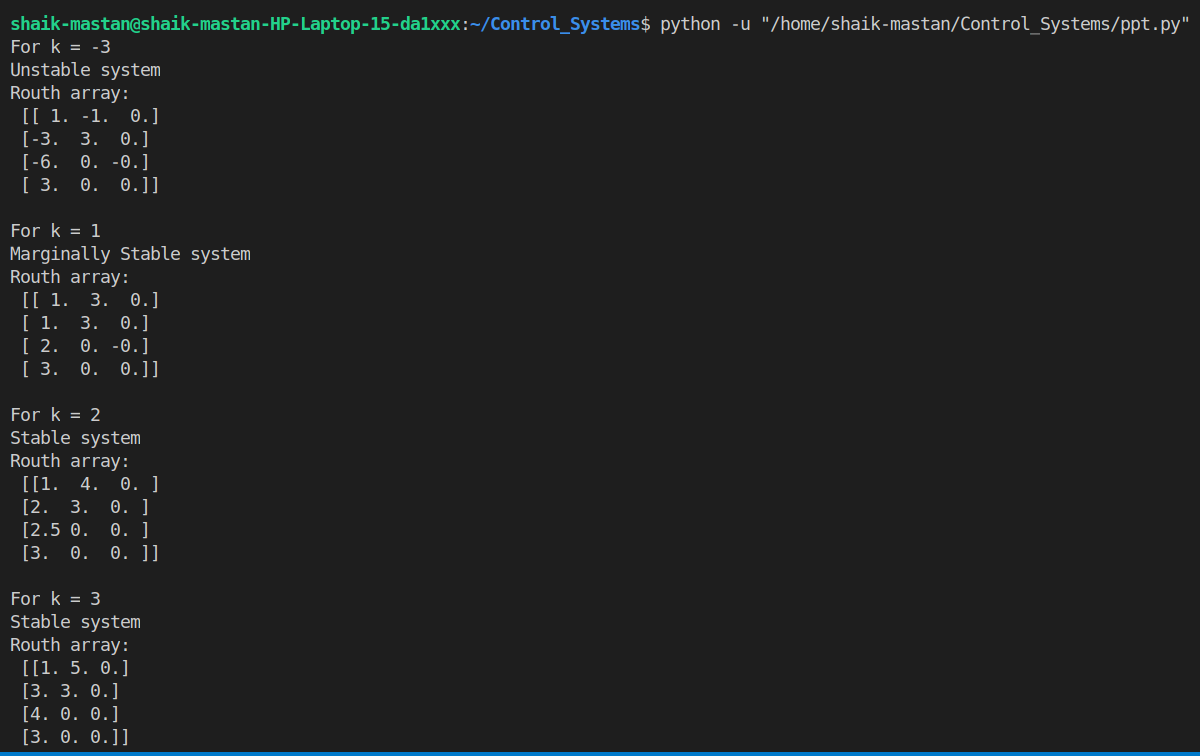
\includegraphics[scale = 0.27]{Terminal.png}
\end{figure}
\end{frame}

\begin{frame}{\textbf{Verification of the solution}}
The poles have been plotted for three different values of k.
\begin{figure}
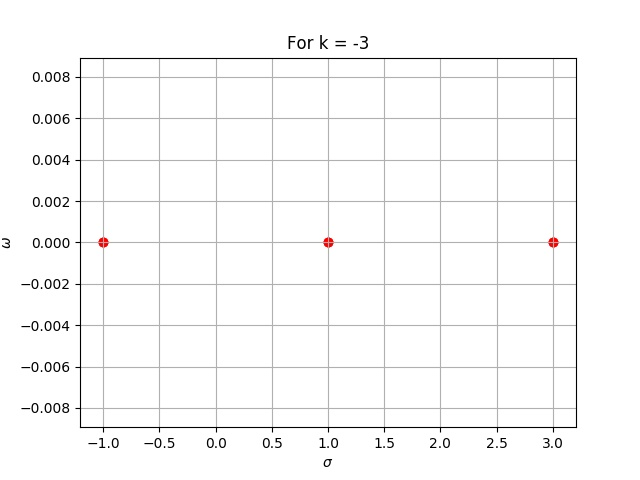
\includegraphics[scale = 0.6]{k=-3.jpg}
\end{figure}
\end{frame}

\begin{frame}
\begin{figure}
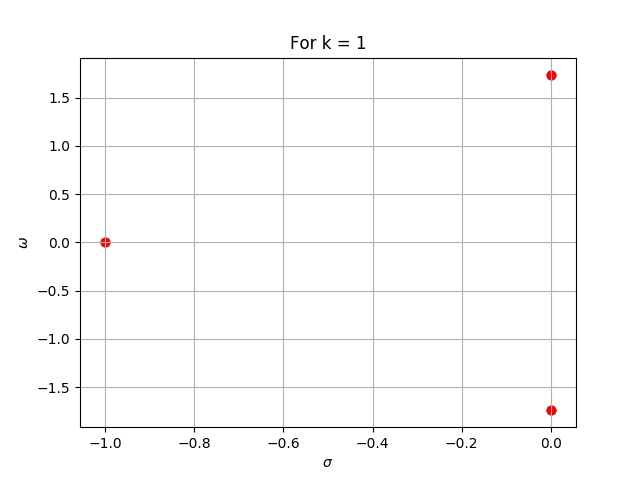
\includegraphics[scale = 0.6]{k=1.jpg}
\end{figure}
\end{frame}

\begin{frame}
\begin{figure}
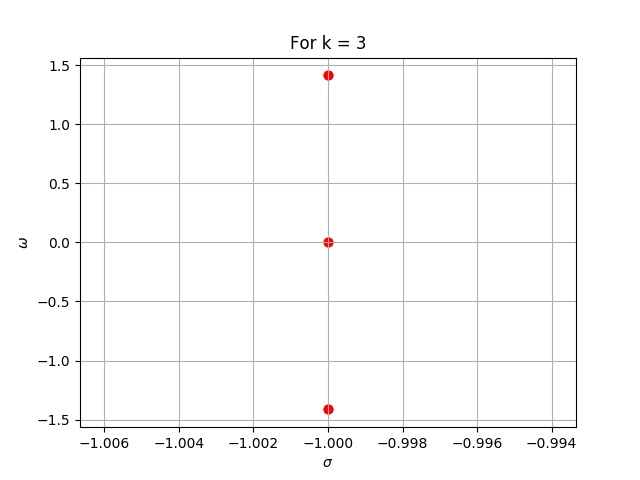
\includegraphics[scale = 0.6]{k=3.jpg}
\end{figure}
\end{frame}
\end{document}

